% Springer LNNS / LNCS proceedings format (llncs class).
% Text is taken unchanged from AI_Red_Team_Honeypot_Springer_Style_Formatted_PLS_LAST_ONE_IMDED.docx.
\documentclass[runningheads]{llncs}
\usepackage[T1]{fontenc}
\usepackage{graphicx}
\usepackage{booktabs}
\usepackage{amsmath}
\usepackage{makecell}
\renewcommand\theadfont{\normalfont}
\usepackage{xurl}
\usepackage{hyperref}
\usepackage{color}
\renewcommand\UrlFont{\color{blue}\rmfamily}
\urlstyle{rm}
\graphicspath{{figures/}}

\begin{document}

\title{Do LLM Red-Team Agents Generate Realistic Honeypot Traffic? A Transfer Study Against Real Cowrie Sessions}
\titlerunning{Do LLM Red-Team Agents Generate Realistic Honeypot Traffic?}

\author{Keshav \and Anshul Sharma \and Parth Kansal \and Virain Nayar}
\authorrunning{Keshav et al.}

\institute{Chandigarh University, Punjab, India\\
\email{keshavc026@gmail.com, anshul08062005@gmail.com, parth.kansal823@gmail.com, nayarvirain1@gmail.com}}

\maketitle

\begin{abstract}
Labeled attack data is hard to come by when building honeypot defenses, so one tempting idea is to let LLM ``red-team'' agents attack a honeypot we control and train on what they do. We tested whether this works. Three LLM attackers (DeepSeek-V3.2, Gemma-3-4B and GPT-OSS-120B) each ran 20 SSH sessions against two Cowrie honeypots: one with the standard shell emulation and one whose output was written by Qwen3-32B. We compared these 120 sessions with 1,672 real interactive sessions from one day of the public CyberLab honeynet. The two sets look very different: their command usage diverges strongly (Jensen-Shannon divergence 0.700 on a 0--1 scale), and a simple classifier separates them perfectly (AUC 1.000). The reason is intent. The agents explored the system and searched for files and credentials, while most real sessions (1,038) ran the same cryptominer dropper. We labeled session intent using two blind, independent LLM annotators, and the authors then cross-verified the labels. A classifier trained on the synthetic sessions reached a macro-F1 of only 0.205 on real sessions, compared with 0.983 when trained on real sessions, and adding the synthetic data to real training data gave no gain (0.981). We also found that GPT-OSS-120B leaked its own chat-format tokens and reasoning text into the shell in 18 of its 40 sessions, which must be filtered out before analysis. With a single ``explore the system'' persona, LLM-agent sessions did not make useful training data for real honeypot traffic.

\keywords{Honeypots \and Cowrie \and large language models \and synthetic data \and dataset shift \and intrusion detection}
\end{abstract}

\section{Introduction}

Honeypots give defenders firsthand information about what the attackers do. A medium-interaction SSH honeypot such as Cowrie \cite{oosterhof2015cowrie} logs the commands the user typed and the files the user downloaded, as well as the passwords which have been entered. These logs can train defensive models. For instance, a classifier for each session can be used to label the session with the primary objective of the session, as in the spirit of MITRE ATT\&CK tactics \cite{strom2018attack}. The problem is supply. Of all the data sessions on our day of CyberLab data \cite{sedlar2020cyberlab} studied, only 1,672 of 76,785 sessions used at least one command. Most of them are repetitions of a few bot scripts.

The solution seems to be a formality for LLM agents. They can be instructed to plan and execute multi-step attacks in recent research \cite{deng2024pentestgpt,fang2024hack}. If we put such an agent on our own honeypot, it will generate sessions at our discretion and they will be cheap. That is another matter whether those sessions are like real attacks. LLMs have robust notions of what a hacker is doing in a capture-the-flag game. The bots that fill real honeypot logs behave differently.

We ask a narrow question. Does a classifier trained on agent-generated sessions work on real honeypot sessions, and if not, where do the two kinds of data differ? If not, then what are the differences between the two? There are two steps in our response. We measure the difference between numbers without labels first. Second, we train and test classifiers on four train-test pairings, with labels from blind LLM annotation, not keyword rules.

Our contributions are as follows.
\begin{enumerate}
\renewcommand{\labelenumi}{\arabic{enumi})}
\item We publish an open pipeline to run LLM attackers against Cowrie, parses the CyberLab export and recreate all the tables described in this paper.
\item We demonstrate label-free separation of agent sessions and expose the difference is in attackers' intent.
\item A 120 session four-way transfer experiment demonstrates that a classifier trained on these synthetic sessions is not successful on real data and that they do not reliably improve the performance of classifiers trained on real data. The study includes 120 synthetic sessions, one day of real data and one attacker persona.
\end{enumerate}

\section{Related Work}

\subsection{Honeypots and Real Attack Data}

Cowrie is a widely deployed SSH and Telnet honeypot that emulates a shell and keeps track of sessions \cite{oosterhof2015cowrie}. Franco et al. surveyed honeypots for IoT and cyber-physical systems \cite{franco2021survey}. There are few public collections of interactive sessions, and one of the few is CyberLab dataset \cite{sedlar2020cyberlab}. Much honeypot traffic comes from bots. Mirai spread by logging into IoT devices with default credentials \cite{antonakakis2017mirai}. The Outlaw botnet brute-forces SSH, scans for new victims and mines cryptocurrency \cite{trendmicro2018outlaw}.

\subsection{LLM Honeypots and LLM Attackers}

shelLM \cite{sladic2023shellm} and HoneyGPT \cite{wang2024honeygpt} replace the shell emulator with an LLM to fool attackers. We instead use such a backend as a target for an LLM attacker. On the offensive side, PentestGPT splits penetration testing into reasoning, generation and parsing modules \cite{deng2024pentestgpt}. GPT-4 agents can hack websites on their own \cite{fang2024hack}, and AutoAttacker automates post-breach steps \cite{xu2024autoattacker}. Cybench tests agents on professional capture-the-flag tasks \cite{zhang2025cybench}. This work asks whether agents succeed. We inquire about their footprints and if they resemble actual intruders.

\subsection{Synthetic Data and Dataset Shift}

Sommer and Paxson point to the gap between research settings and real networks \cite{sommer2010closed}. Arp et al. list pitfalls in security machine learning, such as sampling bias \cite{arp2022dosdonts}. Ring et al. generate network flows with generative adversarial networks \cite{ring2019gan}. Training on one distribution and testing on another is called dataset shift \cite{quinonero2009dataset}. Rabanser et al. compare ways to detect it \cite{rabanser2019failing}; we use the classifier two-sample test \cite{lopezpaz2017c2st} Gilardi et al. found that ChatGPT beat crowd workers on several text annotation tasks \cite{gilardi2023chatgpt}, which is related evidence that LLM annotation can be reliable.

\section{System and Data}

\subsection{Attacker Agent}

We have a harness that opens an interactive shell on the honeypot. At each turn, the attacker model sees the system prompt and the transcript so far and replies with one shell command. The harness sends it, waits until the output goes quiet, and logs the command, output and latency. A session ends when the model says it is done, hits a turn or time limit, or loses its connection. A command such as a recursive \texttt{find /} could stall Cowrie for minutes, so the harness probes the honeypot before each session and retries failed ones.

The system prompt calls the exercise an authorized research task against a fake, sandboxed machine. It asks the model to act like an intruder who has just gained a shell: look around, search for data or credentials, and consider persistence. All 120 sessions use this one ``explore the system'' persona. This isolates model and backend effects.

\subsection{Attackers and Honeypot Backends}

Our three attackers vary in size, vendor and open-ness: DeepSeek-V3.2 \cite{deepseek2025v32}, Gemma-3-4B \cite{gemmateam2025gemma3} and GPT-OSS-120B \cite{openai2025gptoss}. The static backend is stock Cowrie with its built-in shell emulation. The dynamic backend forwards each command to Qwen3-32B \cite{yang2025qwen3}, which writes the shell output. We ran 20 sessions per attacker--backend cell, 120 in total.

\subsection{Real Data}

Our actual data comes from the CyberLab honeynet dataset \cite{sedlar2020cyberlab}, distributed with CC BY 4.0 license and hash of source IP addresses. The daily file for 2019-11-15 holds 76,785 sessions. Only 1,672 contain at least one command, and we keep only those. One pitfall affects anyone who reuses this data. The export is not Cowrie's native JSON-lines log, but one JSON array that maps session IDs to event lists. Commands sit in the \texttt{message} field as \texttt{CMD: <command>}, not in the \texttt{input} field. A parser for native Cowrie logs therefore reads zero sessions and raises no error.

\section{Methodology}

\subsection{Normalization and Behavior Templates}

Real traffic is repetitive and predictable. Many hosts are using the same bot script, using various URLs, IP addresses and random passwords. To compare behaviors instead of instances we normalize individual instances by masking values specific to a particular session. These are URLs, IP addresses and port numbers, quoted strings, long hexadecimal strings, random alphanumeric tokens and bare numbers. Additionally, we mask the random five-letter tag printed by Mirai-family bots, which is \texttt{/bin/busybox}. A behavior template is used for two sessions with identical sequences of normalized commands. A template deduplication keeps one session per template. It will take 1,672 real sessions down to 22 templates and all 120 synthetic sessions will remain separate. The effective real sample size is therefore 22. A few scripts dominate the per-session view and thus we report real-data results per session as well as per template.

Before any analysis, we remove leaked chat-format tokens from synthetic commands, together with the reasoning text that follows them (Section~\ref{sec:behavior}).

\subsection{Label-Free Measures}

We have three measures that do not require labels. The first is a tactic profile. Each command segment is matched using a regular expression to zero or more of the nine categories aligned with MITRE ATT\&CK \cite{strom2018attack}. They consist of discovery, credential access, account manipulation, persistence, privilege escalation, defense evasion, ingress tool transfer and execution and resource hijacking. The percentage of sessions spent on each tactic, one or more times. The tagger is just a description and not a tag for training data.

The second one is a comparison of the first word of every command segment (for example \texttt{ls} or \texttt{wget}). Verbs distributions are compared using Jensen-Shannon divergence (JSD) \cite{lin1991jsd}. The base-2 version ranges from 0 (if the distributions are identical) to 1 (if there is no common verb in the distributions). We do the resampling with replacement and recompute JSD many times to get a 95\% confidence interval. In addition, we present the Jaccard index for the two verb vocabularies. It is the ratio of the number of common, different verbs to the number of all different verbs. Coverage is the percentage of real verb occurrences whose verb also occurs in the synthetic data.

The third is a classifier two-sample test (C2ST) \cite{lopezpaz2017c2st}. We train a classifier to distinguish the two corpora; when it fails to outperform chance it turns out that the two corpora are very similar. The area under the ROC curve (AUC) is used for our scoring. Generally a score of 0.5 is indistinguishable and 1.0 is perfectly separable. The classifier uses logistic regression on TF-IDF features, weights each token by its frequency in a session and its rarity across sessions. We are comparing the synthetic sessions to the real sessions that were deduplicated from templates over five repetitions of 5-fold cross validation. We test on full normalized commands and also verbs alone to ensure that paths and arguments do not affect the results.

\subsection{Labels from Blind Dual-LLM Annotation, Verified by the Authors}

The transfer experiment needs intent labels. We take them from LLM annotators, because keyword rules can mislead. Mirai-family bots run a bare \texttt{tftp; wget} only to check that the tools exist, then read an ELF header with \texttt{dd} to learn the CPU type and exit. A keyword rule calls this a download (our tagger requires an argument), but both LLM annotators correctly called it recon. Our rubric has eight labels for the primary intent of a session. They are recon, credential access, privilege escalation, persistence, malware drop, resource hijacking, defense evasion and other. Annotators judge the whole command sequence and choose one label. When a session shows several behaviors, a tie-break picks the goal that progressed furthest. The order is resource hijacking, malware drop, persistence, privilege escalation, credential access, defense evasion, recon and finally other.

The set of annotations contains 184 items: the 64 different real command sequences and all 120 synthetic sessions. The 64 real sequences were different at least before we masked the busybox tag; they are in the 22 templates. The items were mixed up and the source of the items was concealed. The two annotators were Anthropic's Claude Sonnet 5.5 and Claude Opus 5.5. Each labeled every item separately, without seeing the other's labels or the item's source. An adjudicator, a third and separate instance of Claude Opus 5.5 that was also blind to the source, resolved every disagreement. All items in the same template received the same final label. We duplicated each template's label to all real sessions in that template, thus labeling all 1,672 real sessions.

We use Cohen's kappa \cite{cohen1960kappa} to assess agreement. The Kappa coefficient corrects raw agreement for chance that two annotators would get if they were to agree randomly. A kappa value of 1 indicates complete agreement, 0 indicates no agreement above chance. (Section~\ref{sec:threats}).

\textbf{Author verification.} After adjudication, the authors cross-verified the final labels and confirmed them. We paid particular attention to the dota template, because its label sets the class of 1,038 real sessions. All results in Section~\ref{sec:results} use the verified labels.

\subsection{Four-Quadrant Transfer Experiment}

Each session is transformed in a TF-IDF vector of the normalized commands, plus three numbers: the number of commands, the mean of command length, and the percentage of chained commands. Classifier 300: A random forest with 300 trees and balanced class weights. There are four train--test pairings, called quadrants, that are tested.
\begin{itemize}
\item Q1 (synthetic $\rightarrow$ synthetic) uses stratified 2-fold cross-validation within the synthetic data. It shows how learnable the task is when one generator produces both sides.
\item Q2 (real $\rightarrow$ real) uses GroupKFold with five folds within the real data. GroupKFold keeps every session of a template in the same fold, so the model never sees a test template during training. Without this grouping, copies of one bot script would sit on both sides and inflate the score.
\item Q3 (synthetic $\rightarrow$ real) trains on all 120 synthetic sessions and tests on all 1,672 real sessions. This is the zero-shot case that motivates the study. Q3-dedup tests on one session per real template instead.
\item Q4 (real + synthetic $\rightarrow$ real) reuses the Q2 folds but adds all synthetic sessions to each training fold.
\end{itemize}

Reported is the macro-F1 and accuracy pooled over folds. Macro-F1 is the average of each class's F1 score over the classes found in the test set; thus, a rare class has a significant effect. Additionally, there are majority baselines for each quadrant that always predict the most frequently occurring label from its training data.

\section{Results}\label{sec:results}

\subsection{Attacker Behavior and Honeypot Backends}\label{sec:behavior}

The three attackers behaved quite differently under the same prompt (Table~\ref{tab:attackers}). On the static honeypot, DeepSeek-V3.2 ran the shortest sessions (13.5 turns on average) and Gemma-3-4B the longest (21.0). GPT-OSS-120B issued 280 unique commands, against 158 for Gemma-3-4B and 124 for DeepSeek-V3.2. It was also the most interested in secrets. Of its static-backend commands, 48.5\% matched our credential keywords, against 27.4\% for DeepSeek-V3.2 and 11.0\% for Gemma-3-4B. Its privilege-escalation share was 13.8\%, against 6.9\% for Gemma-3-4B and 0.7\% for DeepSeek-V3.2.

\begin{table}[t]
\caption{Attacker behavior on static Cowrie and the LLM-backed dynamic honeypot (Qwen3-32B), 20 sessions per cell. Recon/credential values are percentages of commands and may overlap. Latency is mean time until output goes quiet; change is relative to static. Status order: completed / turn limit / connection lost / LLM error / refused / timed out.}\label{tab:attackers}
\centering
\setlength{\tabcolsep}{2pt}
\resizebox{\textwidth}{!}{%
\scriptsize
\begin{tabular}{@{}lccccccc@{}}
\toprule
\thead[l]{Attacker /\\backend} &
\thead{Mean turns /\\total\\commands} &
\thead{Recon /\\credential\\commands (\%)} &
\thead{Latency (s) /\\change} &
\thead{Leak\\sessions} &
\thead{Status\\counts\\(C/M/L/E/R/T)} &
\thead{JSD to real\\{[95\% CI]}} &
\thead{Tactic\\match} \\
\midrule
\makecell[l]{DeepSeek-V3.2 /\\Static}    & 13.5 / 270 & 44.4 / 27.4 & 4.40 / ---       & 0  & 19/0/0/0/1/0 & \makecell{0.783\\{[0.771, 0.810]}} & 5 \\
\makecell[l]{DeepSeek-V3.2 /\\Qwen3-32B} & 16.9 / 337 & 46.3 / 34.4 & 3.65 / $-$17.1\% & 0  & 20/0/0/0/0/0 & \makecell{0.785\\{[0.769, 0.814]}} & 5 \\
\makecell[l]{Gemma-3-4B /\\Static}       & 21.0 / 420 & 57.4 / 11.0 & 4.43 / ---       & 0  & 11/8/0/0/0/1 & \makecell{0.798\\{[0.785, 0.826]}} & 5 \\
\makecell[l]{Gemma-3-4B /\\Qwen3-32B}    & 18.5 / 370 & 47.8 / 20.0 & 2.38 / $-$46.3\% & 0  & 18/2/0/0/0/0 & \makecell{0.746\\{[0.732, 0.778]}} & 7 \\
\makecell[l]{GPT-OSS-120B /\\Static}     & 19.5 / 390 & 54.9 / 48.5 & 4.42 / ---       & 11 & 3/17/0/0/0/0 & \makecell{0.741\\{[0.730, 0.764]}} & 5 \\
\makecell[l]{GPT-OSS-120B /\\Qwen3-32B}  & 16.2 / 325 & 39.4 / 65.2 & 5.51 / +24.8\%   & 7  & 4/0/10/6/0/0 & \makecell{0.746\\{[0.734, 0.780]}} & 7 \\
\bottomrule
\end{tabular}}

\vspace{4pt}
\parbox{\textwidth}{\scriptsize JSD is the verb-distribution divergence to template-deduplicated real data [95\% confidence interval]. The tactic-match column counts tactics (out of nine) whose presence or absence matches the real data.}
\end{table}

The credential share was higher on the LLM-backed honeypot for all three attackers (Fig.~\ref{fig:attackers}). The credential share rose from 27.4\% to 34.4\% for DeepSeek-V3.2 and from 11.0\% to 20.0\% for Gemma-3-4B. For GPT-OSS-120B it rose from 48.5\% to 65.2\%. The dynamic backend was not uniformly slower. Mean latency fell by 17.1\% for DeepSeek-V3.2 and by 46.3\% for Gemma-3-4B, and it rose by 24.8\% for GPT-OSS-120B. Our latency is the time until the honeypot's output goes quiet, thus depending on the sequence of our commands sent by each attacker. We did not distinguish these effects.

\begin{figure}[t]
\centering
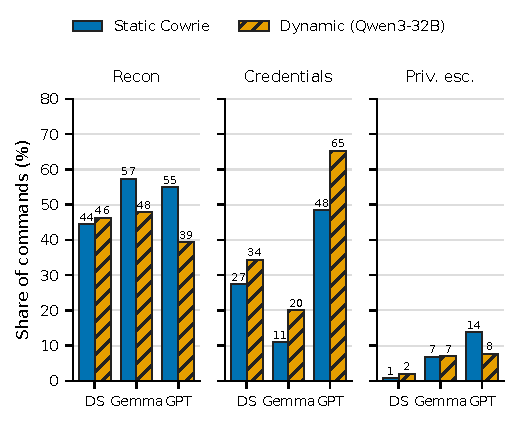
\includegraphics[width=0.75\textwidth]{fig_attackers}
\caption{Share of commands that match each keyword category, per attacker and honeypot backend. DS = DeepSeek-V3.2, Gemma = Gemma-3-4B, GPT = GPT-OSS-120B. Static: stock Cowrie. Dynamic: Cowrie backed by Qwen3-32B. A command can match several categories.}\label{fig:attackers}
\end{figure}

Sessions also closed in various ways. DeepSeek-V3.2 finished on its own in 19 static and 20 dynamic sessions; it refused once. Gemma-3-4B reached the turn limit in 8 static sessions, and timed out once. GPT-OSS-120B made it to the turn cap in 17 out of the 20 static sessions. On the dynamic backend it was the least successful attacker: 10 sessions lost the SSH connection, 6 ended with a LLM error and only 4 completed. It never refused.

In 18 out of 40 of its sessions (11 static, 7 dynamic), GPT-OSS-120B leaked tokens of the chat format into the shell. These are control tokens in its own template for a chat message, e.g. \texttt{<|channel|>analysis<|message|>}, followed by the model's own private reasoning. Our harness treated the whole reply as a command and typed it into Cowrie. This was not the case for DeepSeek-V3.2 and Gemma-3-4B. If left in place, the leaks would change long English sentences for shell prompts and distort every statistic we report. We remove the tokens and the text following the tokens. There are some text strings that leaked due to lack of a separator between the model and the commands.

\subsection{Synthetic Versus Real Data Without Labels}

Real traffic is dominated by a few scripts, while every synthetic session is unique. For real interactive sessions, the 5 most common templates cover 96.2\% of all interactive sessions, while for synthetic sessions, it is only 4.2\%. Real commands are also longer (53.3 compared to 43.0 characters on average) and chained more often (40.3\% against 19.4\%). The length of the median sessions is comparable as well, at 23.0 real and 18.0 synthetic commands.

The biggest real template is alone covers 1,038 of 1,672 sessions. It includes CPU core counting, resets the root password with \texttt{chpasswd}, checks memory and the CPU model and removes old dota files. It then decodes and runs a base64-encoded shell script. The script unpacks a \texttt{dota.tar.gz} archive into a hidden directory under \texttt{/tmp}, starts an SSH scanner against private address ranges and runs the kit's setup script. This falls in line with what Trend Micro attributes to Outlaw \cite{trendmicro2018outlaw}.

There is very little similarity in the tactic profiles (Fig.~\ref{fig:tactics}). All synthetic sessions involved discovery (100.0\%), and almost all synthetic sessions involved credential access (97.5\%). Other common probes included privilege escalation (40.0\%) and persistence (18.3\%). The real sessions were almost absent credential access, persistence and privilege escalation at 1.2\%, 0.4\% and 0.1\% respectively. Real sessions on the other hand performed execution (98.1\%), account manipulation (89.4\%), and resource hijacking (87.9\%). The synthetic shares for these were 6.7\%, 34.2\% and 0.0\%. Both sides employ the same tactic: discovery, with 100.0\% to 92.2\%.

\begin{figure}[t]
\centering
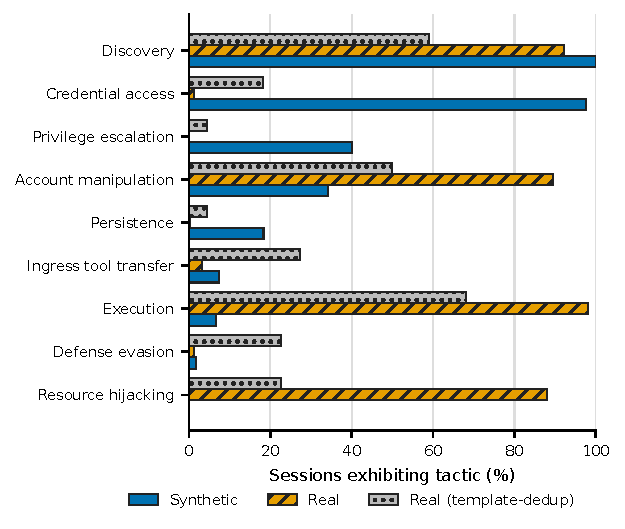
\includegraphics[width=0.75\textwidth]{fig_tactics}
\caption{Share of sessions that touch each ATT\&CK tactic at least once, for synthetic sessions (120), real sessions (1,672) and template-deduplicated real sessions (22).}\label{fig:tactics}
\end{figure}

The template view is less extreme. Counted once per template, real discovery drops to 59.1\%, execution to 68.2\% and resource hijacking to 22.7\%. Thus, a small number of scripts are repeated over and over, resulting in high share usage at the session level. So, there are a few highly-used scripts at the session level. Neither view looks like the synthetic profile.

The verb distributions are far apart. The JSD between synthetic and real verbs is 0.700 (95\% CI 0.688--0.717). Against template-deduplicated real data it is 0.729 (0.719--0.745). The two vocabularies have a Jaccard index of only 0.285. However, 82.0\% of real occurrences of verbs are covered by the synthetic vocabulary. The agents are familiar with the commands, they use them in different proportions and for different things. The top synthetic verbs browse files: \texttt{ls} (712), \texttt{cat} (606), \texttt{head} (243) and \texttt{find} (217). The top real verbs process text and fingerprint the system: \texttt{grep} (8,880), \texttt{cat} (8,123), \texttt{echo} (6,964) and \texttt{uname} (4,437).

The difference between the two corpora is almost complete, as they can be easily separated by a simple classifier. The C2ST AUC is 1.000 $\pm$ 0.000 on normalized commands and 0.996 $\pm$ 0.010 on verbs alone. The verb-only result indicates that separation does not depend paths or arguments. Near perfect separation doesn't mean all downstream tasks will fail, it is a good warning.

All six attacker--backend cells stay far from real traffic (Fig.~\ref{fig:jsd}). Their JSD to the real data that is deduplicated in the template ranges from 0.741 to 0.798. Only the intervals for Gemma-3-4B do not overlap with the rest: JSD 0.746 (on the dynamic backend), compared with JSD 0.798. The dynamic value is slightly higher and intervals overlap for DeepSeek-V3.2 (0.785 vs 0.783) and GPT-OSS-120B (0.746 vs 0.741). The GPT-OSS-120B dynamic cell also ended differently, mostly in lost connections and LLM errors. The number of tactics (out of 9) whose presence or absence matches real data rose from 5 to 7 for both Gemma-3-4B and GPT-OSS-120B. We ran 20 sessions per cell and did not correct for multiple comparisons, so we make no claim about a statistically significant ordering of the cells.

\begin{figure}[t]
\centering
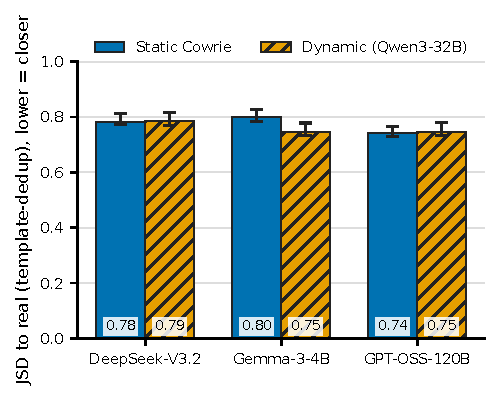
\includegraphics[width=0.75\textwidth]{fig_condition_jsd}
\caption{Verb-distribution JSD between each attacker-backend cell and template-deduplicated real traffic, with 95\% bootstrap confidence intervals. Lower values are closer to real traffic.}\label{fig:jsd}
\end{figure}

\subsection{Transfer Between Synthetic and Real Data}\label{sec:transfer}

Almost disjoint label sets (Table~\ref{tab:transfer}(b)) exist between synthetic and real data. All but a handful of synthetic sessions are mostly credential access 72.5\% (87 of 120). Most of the real data is resource hijacking (1,040) and persistence (443). Resource hijacking never occurs in the synthetic data. Credential access and privilege escalation never occur in the real data. The second-largest real template shows how thin some boundaries are. It performs the same fingerprinting as the dota dropper and changes a password using \texttt{passwd}. It does not contain any payload to unpack, thus it is marked with persistence.

\begin{table}[t]
\caption{Transfer results and final label counts. Labels come from blind dual-LLM annotation and were cross-verified by the authors. Real labels are copied from 22 templates, so the effective real sample size is 22. Q2 and Q4 use GroupKFold by template. For Q1, Q2 and Q4, $n_{\mathrm{train}}$ is the mean training size per fold and $n_{\mathrm{test}}$ counts pooled out-of-fold predictions. F1 is macro-F1 over classes present in the test set; defense evasion and other were never assigned.}\label{tab:transfer}
\centering
\scriptsize
\textbf{(a) Transfer quadrants}\\[3pt]
\setlength{\tabcolsep}{3pt}
\begin{tabular}{@{}llrrcccc@{}}
\toprule
Q & Train $\rightarrow$ test & $n_{\mathrm{train}}$ & $n_{\mathrm{test}}$ &
\thead{Classifier\\F1} & \thead{Classifier\\Acc.} & \thead{Majority\\F1} & \thead{Majority\\Acc.} \\
\midrule
Q1       & Synthetic $\rightarrow$ synthetic        & 60    & 120   & 0.493 & 0.758 & 0.168 & 0.725 \\
Q2       & Real $\rightarrow$ real                  & 1,337 & 1,672 & 0.983 & 0.992 & 0.001 & 0.001 \\
Q3       & Synthetic $\rightarrow$ real             & 120   & 1,672 & 0.205 & 0.022 & 0.000 & 0.000 \\
Q3-dedup & Synthetic $\rightarrow$ real, dedup.     & 120   & 22    & 0.071 & 0.045 & 0.000 & 0.000 \\
Q4       & Real + synthetic $\rightarrow$ real      & 1,457 & 1,672 & 0.981 & 0.992 & 0.001 & 0.001 \\
\bottomrule
\end{tabular}

\vspace{8pt}
\textbf{(b) Final label counts}\\[3pt]
\begin{tabular}{@{}lrrr@{}}
\toprule
Label & Synthetic & Real sessions & Real templates \\
\midrule
Recon                & 14  & 137   & 8  \\
Credential access    & 87  & 0     & 0  \\
Privilege escalation & 2   & 0     & 0  \\
Persistence          & 11  & 443   & 5  \\
Malware drop         & 6   & 52    & 6  \\
Resource hijacking   & 0   & 1,040 & 3  \\
\midrule
Total                & 120 & 1,672 & 22 \\
\bottomrule
\end{tabular}
\end{table}

The inter-annotator agreement was good between the two annotators. The raw agreement was 0.935 and Cohen's kappa was 0.898 for all 184 items. The kappas was 0.873 on real items, and the synthetic items kappas were 0.835. The annotators agreed on 172 items, and the adjudicator resolved the other 12. The most frequent split was recon against credential access, on synthetic sessions that read sensitive files while exploring. One issue is far more important than any other. On the dota template, one annotator chose malware drop and the other chose resource hijacking. The adjudicator chose resource hijacking with the rubric's tie-break. That single decision sets the label of 1,038 real sessions. This decision was reviewed by the authors and confirmed.

The real-to-real classification has been easy and the synthetic-to-synthetic classification has been moderate (Table~\ref{tab:transfer}(a)). Q1 reaches a macro-F1 of 0.493 and an accuracy of 0.758, above its majority baseline of 0.168 and 0.725. Only 60 sessions of Q1 are trained in each fold and 2 out of its classes have 6 or fewer examples. The macro-F1 for the test set of templates the model was not trained on and Q2 reaches 0.983 and the accuracy is 0.992. We take Q2 to be an upper limit. Scripts that are close to each other can create different templates in different folds, and real templates that are the same label may share most of their commands.

By construction, the majority baselines for Q2 and Q4 are close to zero (0.001). GroupKFold is a case of having all the dota template in one test fold with the training majority as persistence. In the other folds the training majority is resource hijacking, which hardly occurs in their test sets.

However, training on synthetic data does not work on real data. Q3 reaches a macro-F1 of 0.205 and an accuracy of 0.022. The figures with one session per template (Q3-dedup) are 0.071 and 0.045. In the real labels, no labels belong to the synthetic majority class, \emph{credential access}, which the model labels 1,636 of the 1,672 sessions. It only has one class the model recognizes: \emph{malware drop}, with a F1 of 0.818 per class. The entire macro-F1 is from that one class, as all others score 0.000. Most of the baseline scores are identical, 0.000, for the same reason: They always predict \emph{credential access}.

No improvement was observed when synthetic data was added to the real training data. Q4 reaches a macro-F1 of 0.981 against 0.983 for Q2, with the same accuracy (0.992).

To test whether the dota label drives these results, we reran the experiment with all three resource hijacking templates, including dota, labeled malware drop. Q3 stayed near zero (macro-F1 0.021), while Q2 and Q4 reached 0.933 and 0.965. The transfer failure does not depend on this label, and adding synthetic data gives no consistent benefit.

With labels from our keyword rules, Q3 also collapsed (macro-F1 0.000). We do not count this as evidence, because those labels share keywords with the features.

\section{Discussion}

\subsection{The Gap Is About Intent}

Our agents were not unsuccessful at their job, they did a different one. They were asked to be a curious intruder and listed directories, read configuration files, and searched for keys. There are a lot of bots driving our sample day. They profiled the CPU, took over the account and launched a scanner and miner kit \cite{trendmicro2018outlaw}. Nobody asked the agents to act like the dominant real population.

\subsection{What the Transfer Result Means}

The first problem with the failure of the Q3 is that it is a label-space problem. A synthetic trained model can not predict the label of most real sessions in absence of resource hijacking sessions. But \emph{recon} and \emph{persistence}, which bot corpora contain, also score an F1 of 0.000. Synthetic persistence is an intruder writing a reverse-shell cron entry or appending an SSH key. Real persistence is a bot script that changes a password between fingerprinting steps. A potential intruder can create a reverse-shell cron entry, or add an SSH key. If you try to add a real persistence, you have to switch password between fingerprinting steps, that's the bot script to do. The label is the same; the behavior is not. In our setting, more sessions from the same persona are unlikely to close this gap.

\subsection{The LLM-Backed Honeypot}

Qwen3-32B only reduced the divergence for the smallest attacker, Gemma-3-4B. Richer shell output could give the weak attacker more to respond to, but we have not tested this. Even the nearest cell (JSD 0.741) is not close to reality in terms of traffic. The backend also increased the percentage of credential requests made by each attacker. What we actually mean when we're talking about Credential Access is the synthetic majority (87); it is absent from the real labels.

\subsection{Leakage and Next Steps}

If the reply to the model is to be understood as a literal action, it will be typed into the terminal with a harness. The transcript still reads like a session, but a lot of the contents are the model thinking aloud. Pipelines should check each command for known control tokens and record the input response without any line between the command itself and the input response. Future work should try bot-like personas (dropper, cryptominer, credential stuffer). In addition, synthetic honeypot data should be accompanied by shift measures that are not dependent upon the labels.

\section{Threats to Validity}\label{sec:threats}

\textbf{Label quality.} Our labels were first produced by LLMs. The two annotators and the adjudicator are all Claude models from one provider and may share biases. To reduce this risk, the authors cross-verified the final labels for all 184 items and confirmed them. This check has limits. It was done by the authors, who know how the data was built, so it is a consistency check and not an independent blind human annotation, and we did not measure human--human or human--LLM agreement. The most consequential decision is the dota template: the annotators split between malware drop and resource hijacking, the adjudicator chose resource hijacking, and that one label covers 1,038 real sessions. We confirmed it, and relabeling all three resource hijacking templates as malware drop still leaves Q3 near zero (0.021) (Section~\ref{sec:transfer}). An independent human audit by annotators outside the author team remains future work. The full annotation kit is released for anyone who wants to rerun it, including the rubric, the blinded sheets, the annotators' labels and the adjudicator's rationales.

\textbf{Blindness is imperfect.} The annotators did not see any item's source, but the style of LLM-generated commands is recognizable (clean single commands with tidy flags), so an annotator could infer the source and be influenced by it. We cannot measure how often this happened. Our own verification was not blind either.

The synthetic sample is small (20 sessions/attacker--backend cell).

The real data are for 1 day (2019-11-15) on 1 honeynet. One campaign accounts for 62\% of interactive sessions and the top five templates account for 96.2\% of the real sample of effective campaigns. Deduplication has an impact, which reduces the dominance but increases the JSD to 0.729.

The tactic tagger and the keyword shares in Table~\ref{tab:attackers} use regular expressions that we wrote. They might mislabel commands, such as any route that includes \texttt{passwd} may be interpreted as credential access. Changes as big as those shown in Fig.~\ref{fig:tactics} are not likely to be tagger artifacts, but small changes are possible.

In all sessions the model effects are not separated from the persona effects, all sessions use one prompt, three attacker models and one backend model, so persona effects are not separated from model effects. The conclusions relate to these models when operating in this persona, rather than LLM attackers in general. Finally, glued commands can not be repaired by leak stripping and the C2ST applies one family of classifiers. A perfect AUC does not mean there is no other representation that would divide the corpora, but rather that the corpora are separable.

\section{Conclusion}

We questioned if LLM red team agents generate traffic that can be considered as honeypot traffic and whether it matches the characteristics of traffic to be defended. Under one ``explore the system'' persona, the answer in our setting is no. The agents browse files and hunt for credentials, while most real sessions run one cryptominer dropper. The classifier that is trained using these synthetic sessions achieves a macro-F1 of 0.205 for real sessions, compared to 0.983 for the classifier trained with real data. Adding synthetic data does not have any gain (0.981). The LLM ensnared honeypot reduced the difference just for Gemma-3-4B, and all other cells remained well away from actual traffic. Results are based on a small synthetic corpus, one day of data (2019), 22 real behavior templates, one persona and labels generated by an LLM, cross-verified by the authors. Next, we will create personas targeting the bot population, more days and more honeynets, and an independent human audit of the labels. Reporting on synthetic honeypot data should be in the form of contamination checks, including the chat-format leak rate.

\section*{Ethics}

Our own isolated honeypot was the only one targeted by the attacker agents. It holds no real data, and it doesn't have any path to third-party systems. The harness is single-target and lacks scanning and discovery capabilities. The public CyberLab release of real data is CC BY 4.0, where source IP addresses are replaced by hashes. We made no attempt to re-identify any source. We used only session IDs, event timestamps and command text, and the LLM annotators saw only command transcripts. The released version of the code does not have additional attack capabilities beyond the standard post-compromise commands found in public honeypot data.

\section*{Code and Data Availability}

We publish the attacker harness, the CyberLab parser, the normalization and tagging module, and scripts that generate all of the tables and figures. The release also includes the annotation kit---both annotators' labels and the adjudication rationales. The real data are available on Zenodo at \url{https://doi.org/10.5281/zenodo.3687527} \cite{sedlar2020cyberlab}. Every number in this paper is written to a results file by one of the released scripts. This project has also been published on GitHub and can be accessed at \url{https://github.com/parthkansal823/Honeypot_RedTeaming-paper}.

% splncs04_unsrt = Springer's splncs04 with sorting off, so references keep the
% citation-order numbering [1]-[25] of the Word file. Use splncs04 for alphabetical.
\bibliographystyle{splncs04_unsrt}
\bibliography{references}

\end{document}
